\chapter{Methodology}
\label{chapterlabel5}
In order to identify the uncertain modelling assumptions, several models will be run. In this section, the process of evaluating the modelling assumption will be explained as well as the framework of assessing the uncertainties.

\section{Patient data}
The patient data was obtained from the Beijing Institute of Technology. The dataset included several geometries of patient's aorta and flowrate and luminal area waveform at the inlet and the outlets obtained via 4D-Flow MRI and cine-MRI. Additionally it also included the systolic and diasctolic measurement of the patiend and the heart rate of the patient as well. \par 

\section{0D model}
The whole system is initially described as a lumped model or also called the 0D model, where the different properties of the system are made analogous to electronics components. The model assumes that the parameters such as velocity and pressure are uniformly distributed. \par

\begin{figure}[ht!]
  \centering
  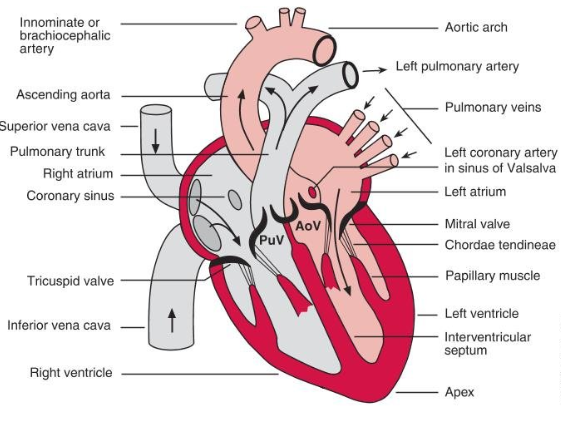
\includegraphics[draft]{Figures/heart}
  \caption{Schematic of the 0D model}
  \label{fig:0d}
\end{figure}

The aorta was divided in sections and which were represented with an elementary building block consisting of an inertance (L) and a resistance (R). The whole system can be seen on the Figure \ref{fig:0d}. The parameters of each section has been obtained from an steady state simulation CFD simulation, where the inlet was the average flow rate at the inlet measured from the 4D-MRI. The parameter were then calculated as:
\begin{align}
    L = \frac{\rho L}{A_{avg}}
\end{align}
\begin{align}
    R = \frac{\Delta P}{Q_{avg}}
\end{align}
where $\rho$ is the density, $L$ is the length of the segment, $A_{avg}$ is the average length of the section, $\Delta P$ is the pressure drop across the section and $Q_{avg}$ is the average flow rate at the section obtained from the patient's MRI dataset.\par

\begin{figure}[ht!]
  \centering
  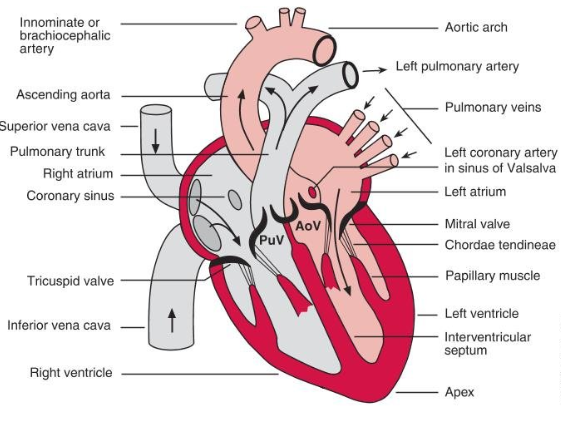
\includegraphics[draft]{Figures/heart}
  \caption{Windkessel models \textbf{a} two-element; \textbf{b} three-element; \textbf{c}} four-element
  \label{fig:wind}
\end{figure}

To account for the elasticity of at the outlet, an electronic analogous model will be used at the outlets, a Windkessel model (different types shown in Figure \ref{fig:wind}). The three-element Windkessel has been chosen for this study. While the two-element Windkessel is easier to implement, it cannot describe well the high frequency effects. The four element Windkessel can describe the impedance characteristics better, however due to the additional forth element, the parameters are difficult to estimate. Thus, the three-element Windkessel (WK3) model is often used theoretical research. \par

\subsection{Parameter tuning}
In order to get accurate parameters for the given pressure measurements and flow rates, an optimization algorithm was used. \par

Initially, the whole system is described as a single WK3 model where the $R_1$ and $R_2$ have been set as a ratio $R_1/(R_1+R_2) = 5.6\%$. Thus, only two parameters need to be fitted. The objective function minimizes the difference between the target systolic and diastolic pressure and the maximum and minimum pressure of the WK3 pressure curve which then gives:
\begin{align}
    min \sqrt{(P_{sys}-P_{max})^2+(P_{dia}-P_{min})^2}
\end{align}
 Additionally, non-negative constraints and bounding constraints have been applied for the parameters between the bounds [0, 2]. \par

Obtaining the parameters for the whole system, the compliance is distributed proportionally to $\bar{Q_i}$ to the outlets and the resistances are set as a ratio as seen previously. Therefore, for each of the outlet, only one parameter needs to be optimized. The objective function sums up the difference in the target and model pulse pressure and also the target and the model mean flow rate and for the parameters a non-negative constraints and bounding constraints as previously. Thus the objective function to be minimizes is as following:
\begin{align}
    min \sqrt{(P_{sys}-P_{max})^2+(P_{dia}-P_{min})^2+\sum_{i}(\bar{Q}_{i}^{target}-\bar{Q}_{i}^{0D})^2}
\end{align}


\section{Boundary conditions}
The blood is modelled as incompressible with a density 1060 $kg m^{-3}$ and the flow was considered as laminar, which is a common assumption in large arteries \cite{Alimohammadi2014DevelopmentConditions,Bonfanti2017ComputationalData}. The inlet condition was obtained from 4D-MRI and a flow rate was applied.\par

The three-element Windkessel parameters obtained from the 0D model has been coupled to the outlet, thus the mean pressure (P) and the flow (Q) at the outlet are related by:
\begin{align}
    P=(R_1+R_2)Q-R_2C\frac{dP}{dt}+R_1R_2C\frac{dQ}{dt}
\end{align}
where $R_1$, $R_2$ and $C$ are the parameters obtained for each of the outlet. \par

A no-slip condition was applied and the wall were considered as rigid. \par

\section{Modelling assumptions}
Different modelling assumptions can be used while modelling a patient aorta. The choice is often justified by the modeler but the resulting simulations can yield different results. In this section different modelling assumption that were taken into account are discussed and a number of combination of the assumption will be made resulting in 48 different CFD models.

\subsection{Segmentation}
While the patient geometries are obtained from the images, the segmentation criterion can affect the resulting in a varying geometry. While all geometry can be considered valid, this can results in differences in the lumen's area. \par

For the simulations, a two additional geometries will be used, where the patient's aorta is larger and narrower by 0.6 mm which accounts for the variability of the segmentation done (the original patient aorta was segmented from CT scans with 1 mm voxel). \par

\subsection{Image processing}
Depending on the image processing done on the patient scans the resulting geometry can have variation as well. These depend on the choices doing while improving the quality of the scans. \par

In the simulations two different aortas are being used, where one surface is smooth and the other is unsmoothened.

\subsection{Mesh}
While a finer mesh can yield much more accurate results, it comes with a trade-off of computational run time. In CFD simulatons it is a good practice to run mesh sensitivity studies before running the full simulation, however a proper guideline has not been introduced, therefore the decision on the mesh is often left to the modeler.\par

In this project a several meshes have been used to  assess how much the mesh can influence the final results. Four different meshes have been used with ~120,000 ~250,000, ~600,000, and ~1,100.000 elements.\par

\subsection{Viscosity}
As seen in the Chapter \ref{chapterlabel2}, while blood has shearing properties it is often assumed as Newtonian in larger arteries. Another approximation often used in simulations is using the Carreau-Yasuda model. \par

These two blood models will be considered, a Newtonian blood will be modelled with a constant viscosity of 0.004 $Pa s$ and the non-Newtonian blood will be modelled as Carreau-Yasuda model with the parameters taken from the Gijsen et al \cite{Gijsen1999TheModel}.


\section{Validation}